\section{From local to uniform dissipation: the sunburst model}

%{\bf describe a bit the model and the interplay between uniform and local dissipation 
%regime}

\begin{figure}
    \centering
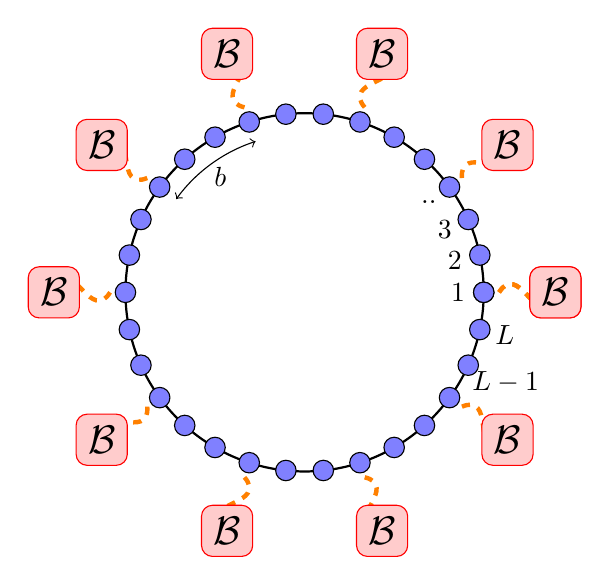
\begin{tikzpicture}[scale=0.65]
    \draw[thick] (0,0) circle (3.5cm);

    \foreach \x in {0,12,...,360}
    \filldraw [fill=blue!50] (\x:3.5cm) circle (0.2);

    \foreach \x in {0,36,...,360}
    \draw[orange, dashed, ultra thick] (\x:3.8cm) .. controls (\x+8:4.2cm) and (\x-8:4.6cm) .. (\x:4.6cm);

    \foreach \x in {0,36,...,360}
    \node[rectangle,
    draw = red,
    text = black,
    fill = red!20!white,
    rounded corners,
    minimum size=0.65cm] (r) at (\x:4.9cm) {\Large $\mathcal{B}$};

    \draw[<->] (108:3.1cm) arc
    [start angle=108,
        end angle=144,
        radius=3.1cm,
    ] ;

    \node[] (s1) at (126:2.8cm) {$b$};

    \node[] (s1) at (0:3cm) {$1$};
    \node[] (s2) at (12:3cm) {$2$};
    \node[] (s3) at (24:3cm) {$3$};
    \node[] (s4) at (36:3cm) {$..$};
    \node[] (s5) at (-12:4cm) {$L$};
    \node[] (s6) at (-24:4.3cm) {$L-1$};
\end{tikzpicture}
    \caption{Sketch of a Kitaev ring with $L=30$ qubits coupled with $n=10$ dissipators in a \textit{sunburst} geometry ($b=3$ in the figure).}
    \label{fig_sketch_sunburst_dissipation}
\end{figure}

We consider a lattice model tailored to unveil the crossover regime between the  dissipation schemes presented. We investigate a $(1+1)$-dimensional Kitaev ring with local particle-decay dissipators arranged in a \textit{sunburst} geometry~\cite{FRV-staticsunburst, FRV-timesunburst, MS-2022-sunburstquench}. The whole apparatus is sketched in Fig.~\ref{fig_sketch_sunburst_dissipation}. The open quantum system is coupled with the environment by means of $n\equiv L/b$ equally-spaced external baths, which reduce to some extent the translation invariance of the starting model.
In particular, we focus on the case of particle-decay jump
operators in the Eq.\eqref{eqlindblad}, i.e., $\hat L_x = \hat c_x$ , where fermionic 
particles are continuously removed from the site $x$. With this choice,
the Liouville operator ${\cal L}$ is quadratic in the fermionic
variables $\hat c_x$ and $\hat c_x^\dagger$ , and, in this sense, we say that the
open ring we study maintains its integrability. Most of
the results discussed in this work should preserve their
validity also for particle-pumping dissipation ( $\hat L_x = c_x^\dagger$ ),
since Eq. \eqref{eqlindblad} is still quadratic in the fermionic creation
and annihilation operators.\\


We explore different large-size limits, depending on the number of dissipators taken into account. A thorough study of the Liouvillian gap $\Delta_\lambda$ is the main focus of the first part of this section. In the second part, we examine the real-time evolution of the system, triggered by a \textit{soft quench} of a coupling constant appearing in the defining hamiltonian~\footnote{In a \textit{soft quench} the variation of the quenched parameter is attenuated down to $0$ with increasing the lattice size $L$.}. Starting the protocol in the proximity of a CQT, we study the out-of-equilibrium dynamic using RG arguments and FSS frameworks~\cite{C-1996-ScalingandRG, RV-2021-coherentanddissipativedynamicsreview}.\\

We emphasize the interplay between the unitary and dissipative dynamics and the role played by the gap $\Delta_\lambda$, extending some of the results already presented in Ref.~\cite{NRV-2019-competingdissipativeandcoherent} to our model. To outline our FSS theory, we mainly focus on the scaling properties of the critical correlations and one of the most common entanglement quantifiers, i.e., the entanglement entropy~\cite{ZMZ-2021-Renyientropiesopen}.



\subsection{Liouvillian Gap}

This section is devoted to discussing the different scaling behaviors observed for the Liouvillian gap $\Delta_\lambda$ defined in the subsection \ref{subsec_liouvilliangap}. We will consider two different limits, depending on the number of dissipation sources considered with increasing the lattice size.

%\vspace{-0.4cm}

\subsubsection{Liouvillian gap at fixed $b$}

The value of the Liouvillian gap at fixed $b$ can be computed using two different algorithm.
One, useful for small value of $b$, consists to analyze the system in the Fourier space 
the Lindblad vectorized Eq. \eqref{vecteqlindblad} whose spectrum gives the gap. 

The latter uses the third quantization technique, see details in 
Ref.~\cite{P-2008-thirdquantization}, particularly convenient for high value of the 
parameter $b$ \cite{franchi2023Liouvillian}. Without loss of generality, we will focus only
on small values of $b$, i.e. up to $b=7$, but all the results can be extended also in
the case of high $b>7$.\\

For $b=3$, the Liouville gap $\Delta_\lambda$ shows a behavior in terms of $w$ in Fig.~\ref{fig_liouvgap3b}.
At fixed $L$, we can easily distinguish two different regimes for the gap, which are separated by a bump in the gap located at $w_*(L)$. We clarify that a non-monotone trend in $\Delta_\lambda$ is not unexpected due to the presence of the \textit{quantum Zeno effect} — the dynamic of a quantum system slows down when it is frequently monitored~\cite{MS-1977-quantumzeno, HHNU-2022-Incoherentons}. Note also that both $w_*(L)$ and $\Delta_\lambda(w_*)$ vanish in the thermodynamic limit, so only the region with $w\geq w_*$ is relevant to determine the typical relaxation time of the system for large enough ring sizes. As shown in Fig.~\ref{fig_liouvgap3b}, for $w<w_*$, the gap is perfectly compatible with a linear dependence of the form

\begin{figure}[!h]
    \centering
    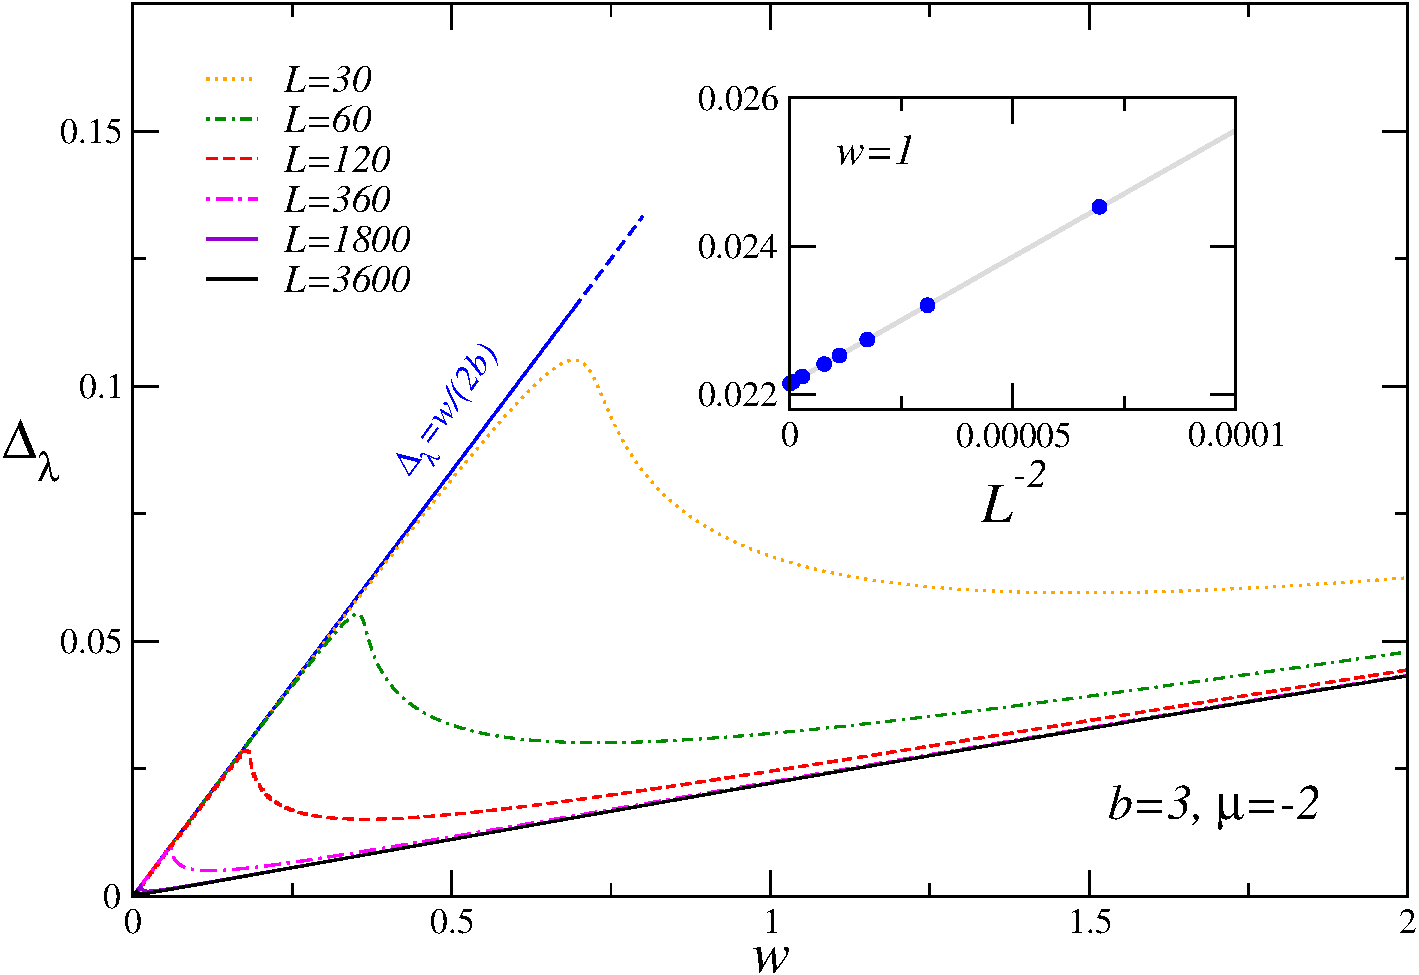
\includegraphics[width=8cm]{imm/gapliouv3b.pdf}
    \caption{Liouvillian gap $\Delta_\lambda$ in terms of the dissipation coupling $w$ for $b=3$ and fixed $\mu=-2$. For small $w$ and $L$ finite, the gap depends linearly on the dissipation strength as $\Delta_\lambda=w/2b$. With increasing $L$ and finite $w>0$, the Liouvillian gap approaches a different regime, which still depends linearly on $w$. In the inset, scaling corrections evaluated at $w=1$ are perfectly consistent with a $L^{-2}$ decaying. The gray straight line is drawn to guide the eye.}
    \label{fig_liouvgap3b}
\end{figure}

\begin{equation}
\Delta_\lambda(w, b)=\frac{w}{2b}\,, \quad w<w_*\,.
\label{eq_deltaL_w_smaller_w*}
\end{equation}

We have verified numerically that the above expression holds also for different values of $b\leq7$ (not shown). This equation has a clear interpretation when we rewrite $\mathbb{D}[\rho]$ in momentum space. Indeed, the full Hilbert space decomposes into the direct product of $n/2$ distinguished sectors with a dimension $4^b$. The effective coupling perceived within each sector is equal to $w/b$. If we additionally assume that the minimum contribution stemming from a single sector is $1/2$ (which is always the case for $b=1$), we get Eq.~\eqref{eq_deltaL_w_smaller_w*}.\\

On the other hand, when $w>w_*$, we observe that the gap $\Delta_\lambda$ still depends linearly on the coupling $w$, but the slope of the asymptotic straight line approached is no longer $1/2b$. We conjecture that for $w>w_*$ and sufficiently large $b$, the following expression describes the Liouvillian gap
\begin{equation}
    \Delta_\lambda(w, b)=A_\mu(b) w\,,\quad A_\mu(b)=\frac{C_\mu}{b^{3}}\,,\quad w>w_*\,,
    \label{eq_liouvillian_gap_largeL}
\end{equation}
where $C_\mu$ is a constant that only depends on the chemical potential $\mu$. Matching arguments with the boundary-dissipation cases surely prompted our guess. Indeed, when $b\propto L$, we expect to recover the leading behavior $\Delta_\lambda\sim L^{-3}$ frequently observed in the literature. Our ansatz is fully supported by the data that we have collected for $A_\mu$ in terms of $1/b^{3}$, as shown in Fig.~\ref{fig_ratelatetime} \footnote{Systematic error bars reported in the figure have been estimated from the comparison of $A_\mu(b)$ for different lattice sizes $L\geq L_{\text{min}}$ and coupling ranges $w\geq w_{\text{min}}$.}. Indeed, a straight line with a slope of $C_\mu=0.601(3)$ describes our data for all values of $b\geq3$ considered ($\chi^2/\text{ndof}=1.0$).  

\begin{figure}
    \centering
    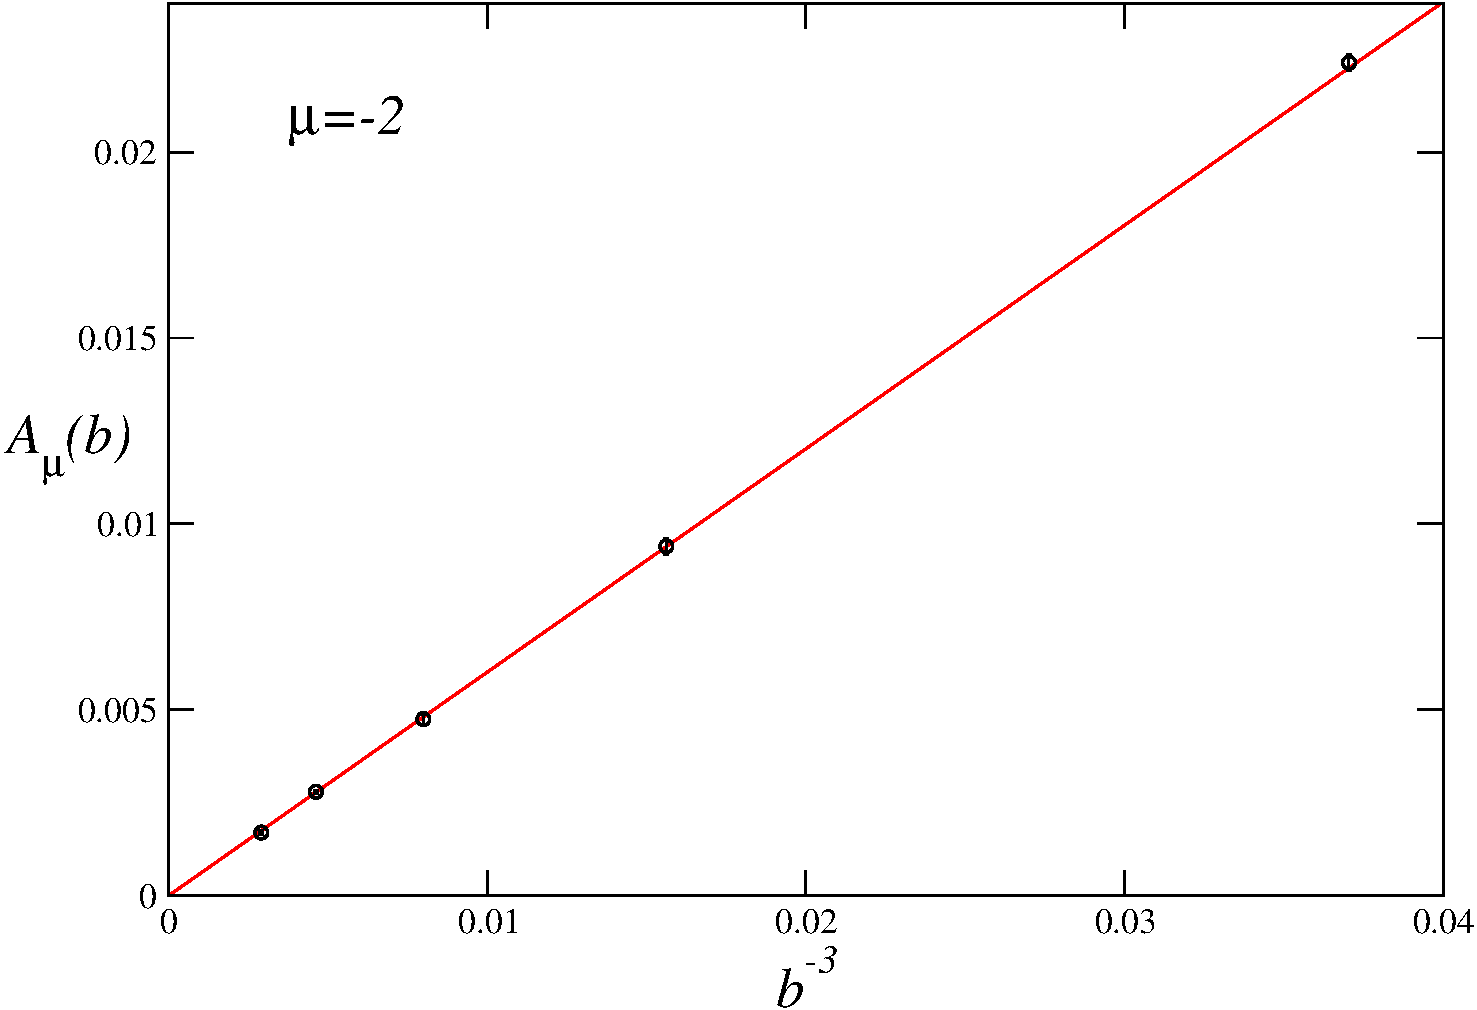
\includegraphics[width=8cm]{imm/ratelatetime.pdf}
    \caption{Liouvillian rate coefficient $A_{\mu}(b)$ versus $b^{-3}$ with constant $\mu=-2$. For $b\geq3$, we observe that $A_{\mu}(b)$ is compatible with a power-law dependence of the form $A_{\mu}(b)=C_{\mu}/b^{3}$, where $C_{\mu}=0.601(3)$ ($\chi^2/\text{ndof}=1.0$).}
    \label{fig_ratelatetime}
\end{figure}

We also want to mention a scaling regime observed for $L\Delta_\lambda$ in terms of $w L$ when the latter quantity is kept fixed in the large size limit. In Fig.~\ref{fig_scaling_delta_apbc}, we report our data for $b=2, \mu=-3$ and $b=4, \mu=-1$.


\begin{figure}[!b]
    \centering
    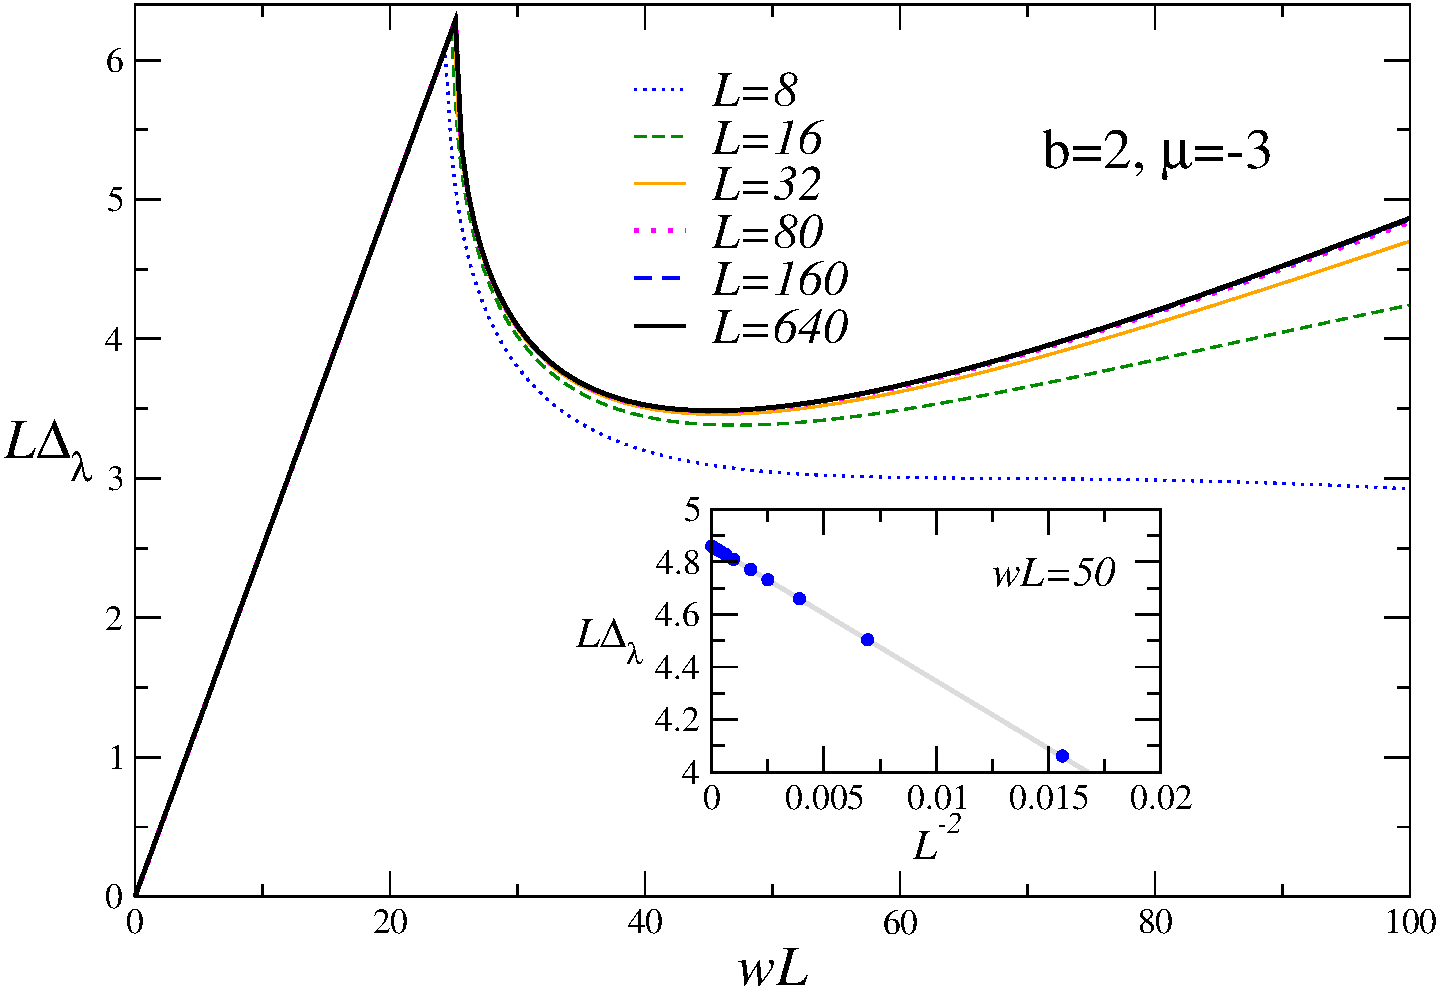
\includegraphics[width=6.4cm]{imm/scalingDeltaapbc.pdf}
    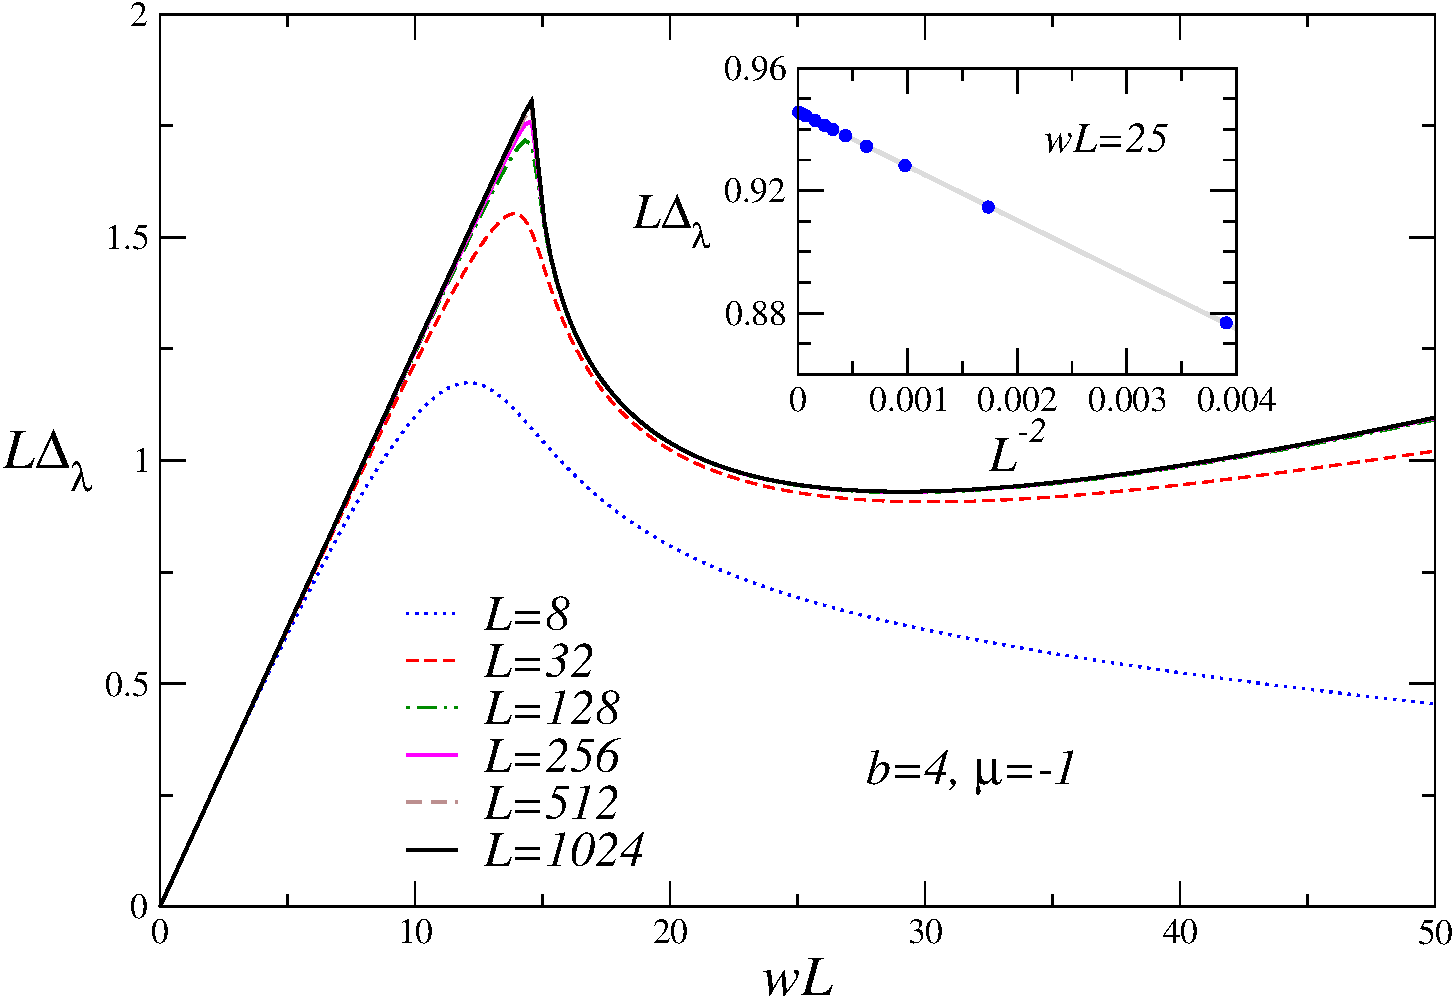
\includegraphics[width=6.4cm]{imm/scalingDelta4bmuminus1.pdf}
    \caption{Scaling of $L \Delta_\lambda$ versus $w L$ for different values of $b$ and $\mu$. On the top panel, we show results for $b=2$ and $\mu=-3$, while on the bottom panel, we fix $b=4$ and $\mu=-1$. The figures show an excellent data collapse in agreement with $L^{-2}$ scaling corrections. The straight lines in the insets are drawn to guide the eye.}
    \label{fig_scaling_delta_apbc}
\end{figure}



\subsubsection{Liouvillian gap at fixed $n$}
\label{sec_liouvillian_gap_fixed_n}

Now we start to study the behavior when we keep $n=L/b$ fixed. Since the number of the
external baths scales with the system size $L$, we will apply the third quantization 
technique, cited above.

The Fig.~\ref{fig_rescaleddelta_apbc_nfixed} shows that the gap scales as  
$\Delta_\lambda\sim L^{-3}$ at fixed $w$ in the regime $w>w_*$ ($w_\star$ is the maximum
point). This scaling is correlated also to the Eq.\eqref{eq_liouvillian_gap_largeL} and
simple matching arguments.\\



\begin{figure}[!t]
    \centering
    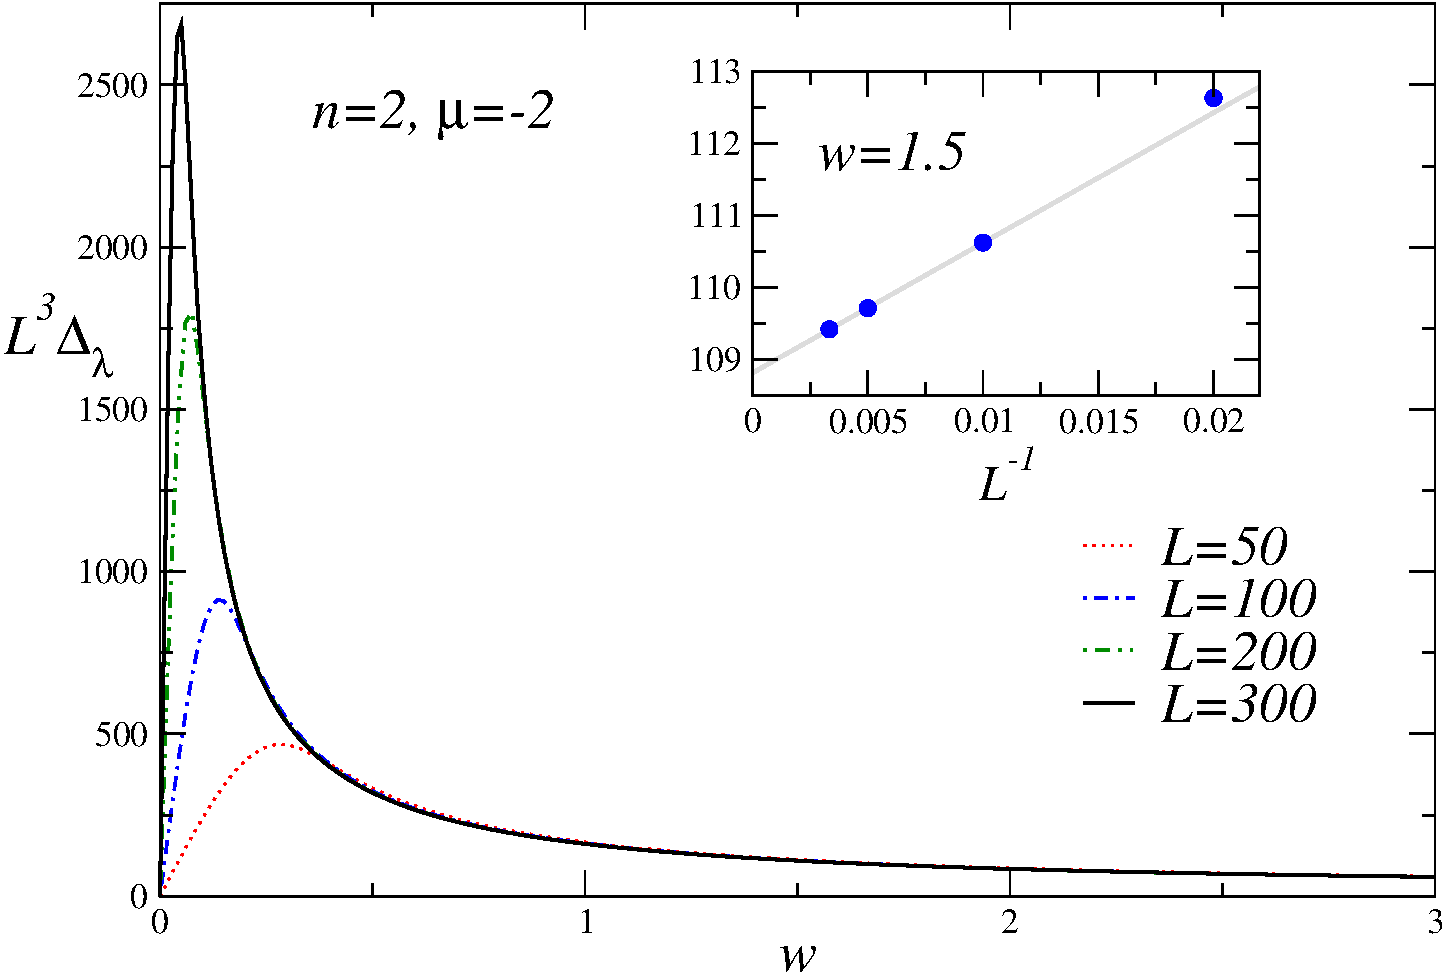
\includegraphics[width=8cm]{imm/delantipk0bl2L3Dw.pdf}
    \caption{Plot of the rescaled gap $L^3\Delta_\lambda$ in terms of $w$ for fixed $n=2$ and $\mu=-2$.  At fixed $w$, the gap shows a nice data collapse within $L^{-1}$ scaling corrections, as provided by the inset for the case $w=1.5$. The straight line is drawn to guide the eye.}
    \label{fig_rescaleddelta_apbc_nfixed}
\end{figure}

\begin{figure}[!b]
    \centering
    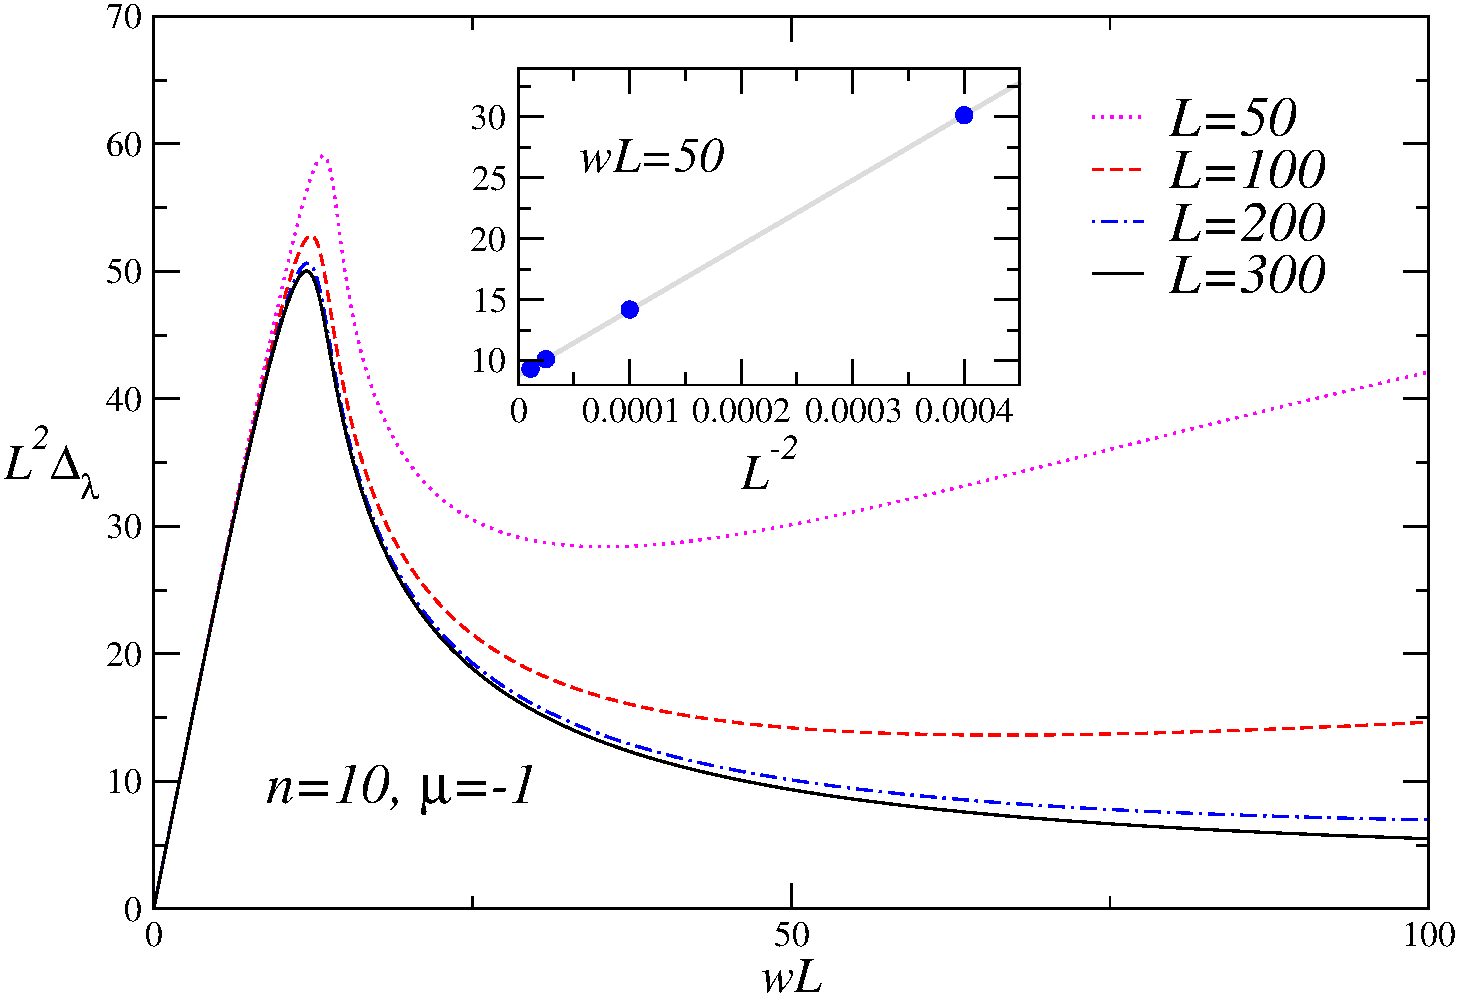
\includegraphics[width=8cm]{imm/scalingDeltanfixedmuminus1.pdf}
    \caption{The figure shows the Liouvillian gap $L^2\Delta_\lambda$ versus $w$ at fixed $n=10$ for $\mu=-1$. In the inset, scaling corrections at $wL=50$ are consistent with a decay $L^{-2}$. The straight line is drawn to guide the eye.}
    \label{fig_scalingDeltanfixed}
\end{figure}

Referring to Fig.~\ref{fig_rescaleddelta_apbc_nfixed}, when $w<w_*$ the gap does not show a uniform limit for $w\to0^+$ as the maximum of $L^3\Delta_\lambda$ grows without bounds with increasing $L$. We shed some light on this peculiar trend in Fig.~\ref{fig_scalingDeltanfixed}, considering the structure of the gap in the proximity of $w=0$ at fixed $n=10$ and $\mu=-1$. In fact, the plot supports the existence of a scaling regime for $L^2\Delta_\lambda$ when $w$ is properly rescaled as $w \sim 1/L$. Scaling corrections are also compatible with a decaying $L^{-2}$, as shown in the corresponding inset. We stress again that numerical results for different values of $\mu$ do not exhibit remarkable differences. We conclude that the different scaling regimes shown by the Liouvillian gap do not depend either on $\mu$ or the quantum phase related to the Kitaev model.


\subsection{Dynamic FSS Framework}


In this section, we study the time evolution of the Kitaev ring in the proximity of a CQT. To this end, we exploit a dynamic FSS framework and use RG arguments to describe the evolution of the critical correlations. Concerning the algorithms adopted, we speed up our simulations by moving to the momentum basis every time we maintain $b$ fixed. On the other hand, when $n$ is fixed, we just monitor the evolution of the two-point correlation functions by solving a closed system of differential equations. To evolve the density matrix $\rho$ in time, we use standard $4^{\text{th}}$-order Runge-Kutta techniques with typical integration time steps of $\Delta t=0.01$.

\subsubsection{The quench protocol and the monitored observables}
\label{sec_observables}

We now present the quench protocol considered to study the time evolution of the open quantum system under scrutiny at CQTs. We prepare the system in the ground state $\ket{\Omega}$ of Eq.~\eqref{kitaev2}. The starting chemical potential $\mu_i$ is always close to the critical value $\mu_c$, meaning that $\abs{\mu_i-\mu_c}\to0$ for $L\to\infty$. At a reference time $t=0$, the ring is driven out-of-equilibrium by suddenly coupling the system with the surrounding environment and eventually quenching the chemical potential to a different value $\mu_i\to\mu_f$. In such a case, the final $\mu_f$ should always be sufficiently close to the critical point. 

We monitor the time evolution of the Kitaev ring by considering two distinguished two-point correlation functions $C(x, y, t)$ and $P(x, y, t)$, defined as
\begin{align}
	C(x, y, t)&\equiv{\rm Tr}[\rho(t)(\hat{c}^\dagger_x\hat{c}_y+\hat{c}^\dagger_y\hat{c}_x)]\,,\\
	P(x, y, t)&\equiv{\rm Tr}[\rho(t)(\hat{c}^\dagger_x\hat{c}^\dagger_y+\hat{c}_y\hat{c}_x)]\,.
    \label{eq_def_two_point_functions_C_P}
\end{align}

%%===============================================================================

\subsection{Out-of-equilibrium FSS frameworks at CQTs with $b$ fixed}
\label{sec_Out-of-equilibrium FSS at CQT}

To describe the time evolution of the system under study at CQTs, we employ RG arguments and a dynamic FSS framework~\cite{C-1996-ScalingandRG, RV-2021-coherentanddissipativedynamicsreview}. The interplay between the unitary and dissipative dynamics of a Kitaev ring subject to complete bulk dissipation ($b=1$) has already been addressed in Ref.~\cite{NRV-2019-competingdissipativeandcoherent}. The results presented in this section extend the FSS reported in that work to all the cases with fixed $b>1$, and provide a complementing discussion on the role of $\Delta_\lambda$ in such a regime. Let us first review the main ideas leading to the FSS theory that we are going to discuss.

When we consider the time evolution of an open quantum system after a quench, analogous equations are more involved given the presence of a larger number of scaling quantities and relevant perturbations. First of all, we need to introduce a pre- and a post-quench scaling field $M_{i/f}=(\mu_{i/f}-\mu_c)L^{y_\mu}$ for $\mu$. In the second place, the time variable $t$ requires a scaling field as well. The most natural guess, which also turns out to be the correct one in most cases, is to rescale $t$ with $L$ on the basis of the dynamic critical exponent $z$. We then introduce the quantity $\Theta$ defined as
\begin{equation}
    \Theta = t L^{-z}\,, \quad z=1\,,
    \label{eq_def_Theta_scaling}
\end{equation}
which is maintained constant in the FSS limit.
Since the number of particle-decay jump operators increases as $L$, we also need to soften the coupling $w$ to observe an interplay between the critical and dissipative modes. We note that the parameter $w$ plays the role of
a decay rate, namely, it is an inverse relaxation time~\cite{NRV-2019-competingdissipativeandcoherent, BP-openquantumsystembook}.
In our work hypothesis, we then suppose that $w$ should be rescaled with $L^{-z}$ to observe universal FSS relations. We introduce the scaling field $\gamma_b$ as
\begin{equation}
    \gamma_b=\frac{wL^{z}}{b}\,,\quad z=1.
    \label{def_gamma_scaling}
\end{equation}
Naturally, the prefactor $b^{-1}$ appearing in $\gamma_b$ is just a matter of convention if one restricts the analysis to just one value of $b$. However, the comparison between different values of $b$ in the FSS limit may add new valuable insights to our analyses. To compare the dissipative processes of different rings on the same footing, we assume that the effective coupling strength is $w/b$. This choice is the most natural one considering the Kitaev ring in momentum space. 

\begin{figure}
    \centering
    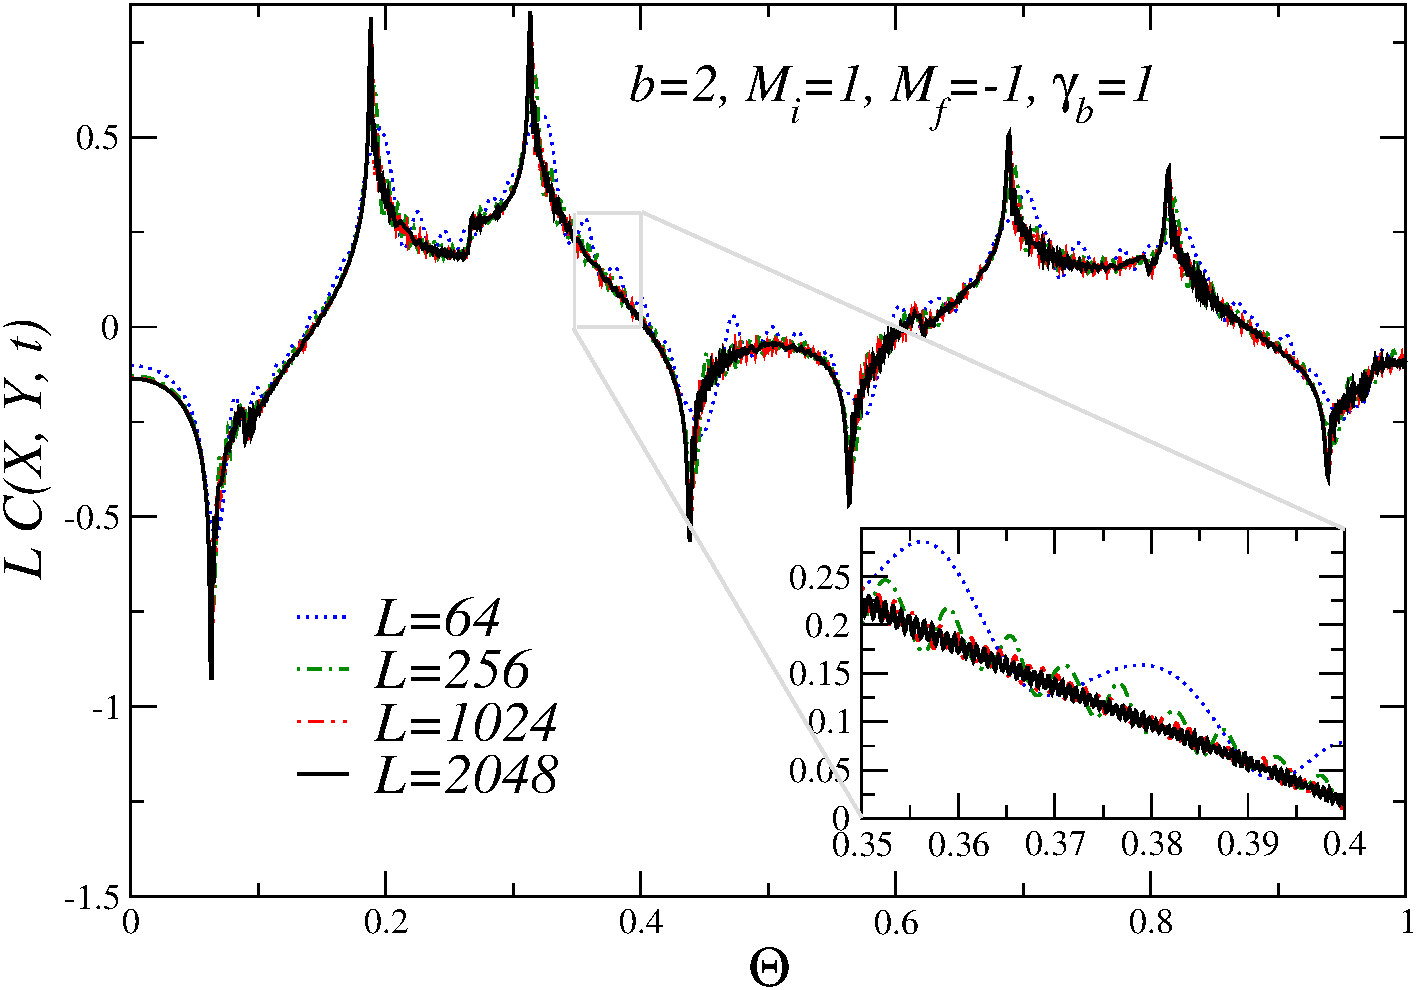
\includegraphics[width=7cm]{imm/Cscaling2b.pdf}
    \caption{Scaling of the two-point function $L C(X, Y)$ in terms of the scaling variable $\Theta$ for fixed $b=2$, $M_i=1$ and $\gamma_b=1$. We consider $(Y-X)/L=1/4$ and fix $x=1$, using translation invariance. In the inset, we show a zoom of the region $\Theta\in[0.35, 0.4]$. Our data clearly support the FSS laws exhibited in Eq.\eqref{eq_scaling_C}.}
    \label{fig_Cscaling2b}
\end{figure}

The universal scaling relations satisfied by the two-point functions $C$ and $P$ in Eq.~\eqref{eq_def_two_point_functions_C_P} follows
\begin{align}
    C(x, y, t) &\approx L^{-2y_c}\mathcal{C}(M_i, M_f, \{X_i\}, \Theta, \gamma_b)    \label{eq_scaling_C}\\
    P(x, y, t) &\approx L^{-2y_c}\mathcal{P}(M_i, M_f, \{X_i\}, \Theta, \gamma_b)\,,
    \label{eq_scaling_P}
\end{align}
where $y_c=1/2$ is the scaling dimension of both $\hat{c}$ and $\hat{c}^\dagger$. 
In Fig.~\ref{fig_Cscaling2b} we show the scaling of $LC(X, Y, t)$ in terms of the scaling quantity $\Theta$ for $b=2$, $M_i=1$, $M_f=-1$, and $\gamma_b=1$. The panel definitely supports the FSS laws exhibited in Eq.~\eqref{eq_scaling_C}. In the inset, we show that the amplitude of the oscillations reduces at fixed $\Theta$ and increasing $L$, roughly as $\sim L^{-1/2}$. We have checked that Eq.~\eqref{eq_scaling_P} holds also for the scaling of the RG invariant quantity $LP(X, Y, t)$ (not shown).  
\subsection{Out-of-equilibrium FSS framework at CQTs with $n$ fixed}
\label{sec_out-of-equilibrium FSS fixed n}

\begin{figure}
    \centering
    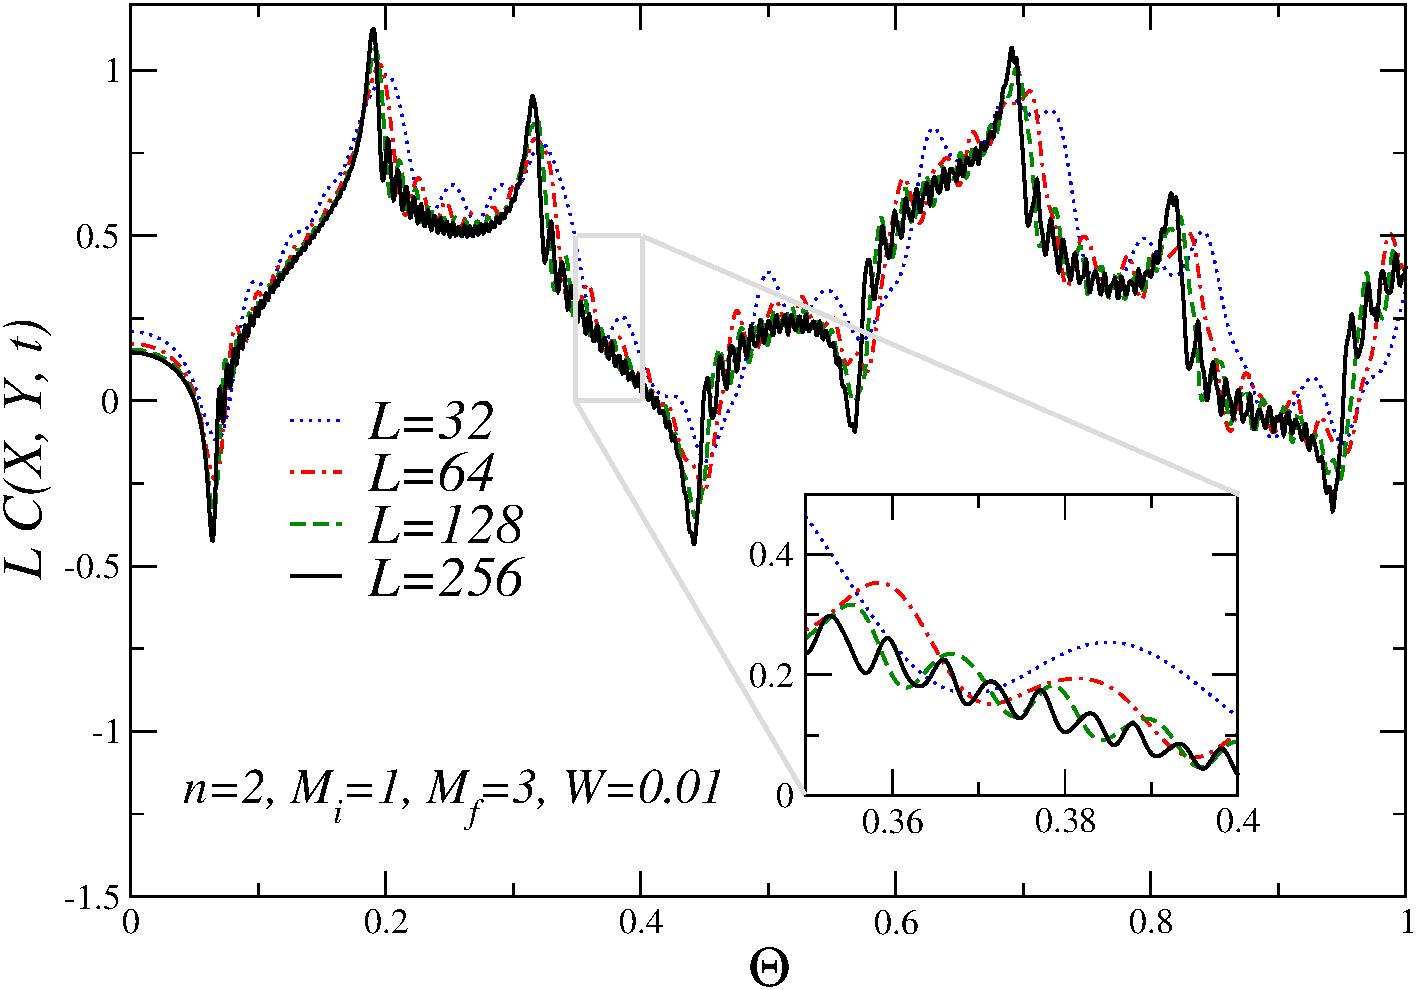
\includegraphics[width=7cm]{imm/fssnfixed2n.pdf}
    \caption{Scaling of the rescaled two-point correlation function $L C(X, Y)$ in terms of $\Theta$ for fixed of $n=2, M_i=1, M_f=3$, and $W=0.01$. We consider $Y-X=L/4$, exploiting translation invariance, and fix the first site to $x=1$ in conjunction with a dissipator. We zoom in on the domain $\Theta\in[0.35, 0.4]$ to emphasize the convergence of different curves with increasing lattice size $L$.}
    \label{fig_fss_2n_fixed}
\end{figure}

In this section, we derive a dynamic FSS framework at CQTs to study the time evolution of Eq.~\eqref{eqlindblad} when the number of the dissipators $n$ is fixed. Most of the scaling relations of the last section are still valid at fixed $n$ with straightforward generalizations. In particular, we just replace the coupling $w$ in our relations, which now represents a decay rate per unit space since $b\sim L$. As a working hypothesis, we expect the scaling field $W$, defined as
\begin{equation}
    W = w L^{z-1}\,, \quad z=1\,,
    \label{eq_def_scaling_variable_W}
\end{equation}
to be a reasonable scaling quantity in the FSS limit. 
For instance, the critical correlations satisfy scaling relations similar to the ones reported in Eq.~\eqref{eq_scaling_C}
\begin{align}
    C(x, y, t)\approx& L^{-2y_c}\mathcal{C}(M_i, M_f, \{X_i\}, \Theta, W)\\
    P(x, y, t)\approx& L^{-2y_c}\mathcal{P}
    (M_i, M_f, \{X_i\}, \Theta, W)\,.
    \label{eq_def_CP_scaling_n_fixed}
\end{align}

We verify our hypotheses in Fig.~\ref{fig_fss_2n_fixed}, showing the scaling curve for $L C(X, Y, t)$ versus the scaling variable $\Theta$ with constant $n=2, M_i=1, M_f=3, W=0.01$. We obtain a nice data collapse considering lattice sizes up to $L=256$. The oscillation amplitudes shrink with increasing $L$, converging to a universal asymptotic curve $\mathcal{C}$. The validity of Eq.~\eqref{eq_def_CP_scaling_n_fixed} has been checked also by inspecting the time evolution of $L P(X, Y, t)$ (not shown).



\begin{comment}
    
\section{Summary}

When we keep $b$ fixed, the gap $\Delta_\lambda$ is always finite and depends linearly on the dissipation strength $w$. Nonetheless, two different regimes emerge for systems of finite size. In the small $w$ region, the gap is given by $\Delta_\lambda=w/(2b)$, whereas, at large $w$ and sufficiently large $b$, it behaves as $\Delta_\lambda=w C_\mu/b^3$. The last equation always controls the gap in the large-size limit and is our starting point to deduce the scaling of such a quantity when $b\propto L$. It is worth mentioning that we also put forward a scaling regime for $L\Delta_\lambda$ as a function of $wL$, which ties together the two different regimes outlined in a smooth manner. On the other hand, when we keep the number of dissipators $n$ fixed, the gap vanishes as $\sim L^{-3}$ at large $L$. Addressing the structure of the gap at small $w$, we find a scaling regime for $L^2\Delta_\lambda$ in terms of $wL$, which is closely related to the presence of a non-uniform convergence of $L^3\Delta_\lambda$ in the limit $w\to0^+$.\\

We develop a dynamic FSS regime at CQTs to describe the time evolution of the Kitaev model under investigation. At fixed $b$, our results extend the FSS theory of Ref.~\cite{NRV-2019-competingdissipativeandcoherent} to the cases with $b>1$. As a working hypothesis, we suppose that the scaling variable associated with the relevant coupling $w$ is $\gamma_b=wL^{z}/b$. Our numerical results for the two-point correlation functions fully support this ansatz. When the number of dissipators $n$ is fixed, the FSS theory outlined at fixed $b$ generalizes straightforwardly after replacing $\gamma_b$ with $W=wL^{z-1}$. 

%In the last section, we analyze the interplay between the Liouvillian gap $\Delta_\lambda$ and the gap related to the Kitaev ring $\Delta$ in the FSS limit. In particular, we take into account the short- and long-time regimes, focusing on how they join together in the FSS limit. When $b$ is fixed, we observe that the link between the two regimes is smooth, whereas, at fixed $n$, the two regions can be easily distinguished given the presence of different power-law scalings for the gaps $\Delta$ and $\Delta_\lambda$. 
\end{comment}


